\documentclass[nofootinbib,pre,superscriptaddress,twocolumn,longbibliography,floatfix]{revtex4-2}
\usepackage{hyperref}
\usepackage{graphicx}
\usepackage{dcolumn}
\usepackage{bm}
\usepackage{amssymb, amsmath}
\usepackage{uri}
\DeclareMathOperator{\realpart}{Re}

\begin{document}

\title{CS229 Project: Detecting Steady States of the Complex Ginzburg-Landau Equation}

\author{Chih-Wei Joshua Liu}
\email{cjoshliu@stanford.edu}
\affiliation{Biophysics Program, Stanford University School of Medicine, Stanford, California 94305, U.S.A.}
\affiliation{Department of Bioengineering, Stanford University, Stanford, California 94305, USA}

\author{Wen-Chieh Chao}
\email{wenj@stanford.edu}
\affiliation{Department of Bioengineering, Stanford University, Stanford, California 94305, USA}

\date{08 November 2024}

\begin{abstract}
    Many physical systems exhibit initial transients, early periods of time in which dynamics are different from those in steady state.
    Some systems important to biological phenomena are characterized by long-lived transients, which may be difficult to distinguish from stationary steady states.
    The complex Ginzburg-Landau (CGL) equation appears in the description of superconductors as well as numerous processes in biological development,
    such as tissue organization and membrane waves.
    The CGL equation's long-lived transients are difficult to distinguish from its steady states.
    Here we examine several machine-learning methods for distinguishing transients from steady states in images of CGL wavefunctions.
    Comparing logistic regression, random forests, and convolutional neural networks (CNNs),
    we find that random forests and CNNs perform well as classifiers of CGL wavefunction stationarity. 
    These findings may be useful in the study of developmental processes described by the CGL equation as well as other systems with long transients.
\end{abstract}

\maketitle

\section{Introduction}
The complex Ginzburg-Landau (CGL) equation
\begin{equation}
    \partial_t A = A + (1+ib)\nabla^2 A-(1+ic)|A|^2 A
    \label{eqn:cgl}
\end{equation}
describes the evolution of a wavefunction $A=|A|\exp(i\phi)$
with both amplitude $|A|$ and phase $\phi$ varying in space and time,
where $\nabla^2$ denotes the spatial Laplacian.
Originally introduced to describe superconductors~\cite{ginzburg1950k},
the CGL equation captures the coarse-grained behavior of all dissipative,
weakly nonlinear U(1) gauge-invariant systems in continuous media under fairly weak assumptions about the nature of diffusion~\cite{aranson2002world}.
In developmental biology, Eq.~\ref{eqn:cgl} arises as a model of Turing patterning~\cite{kuramoto1984chemical},
in which the diffusion of reacting biomolecules gives rise to spatial structures
(such as stripes or spots)~\cite{turing1952chemical}.
In this context, $\realpart(A)$ is the concentration of some biomolecule,
the Laplacian term corresponds to diffusion, and the cubic nonlinearity corresponds to a chemical reaction~\cite{wigbers2021hierarchy}. 

At some biologically relevant values of $c_1$ and $c_2$,
the CGL equation exhibits spiral waves (vortices) that emanate from topological defects (vortex cores)~\cite{tan2020topological}.
At these defects, amplitudes $|A|$ vanish and phases $\phi$ are undefined.
CGL topological defects have $\pm 1$ topological charge (are bosons)
and can anihilate with defects of opposite charge~\cite{liu2021topological}.
Upon initialization from random conditions,
CGL wavefunctions of this regime evolve by a coarsening of vortex domains,
in which defects form and anihilate in often long-lived transients~\cite{chate1996phase}.
The CGL wavefunction eventually settles into a `vortex glass' steady state~\cite{huber1992nucleation},
in which defects have fixed locations and no longer form or anihilate
\footnote{Strictly speaking, defects anihilate at nearly vanishing rates.
This is analogous to the extremely slow but still liquid-like flow of glass materials.}.
Toward the end of a transient, defect anihilation can occur very slowly~\cite{liu2021topological}.
Wavefunctions in late transients and steady states are barely, if at all, distinguishable to the human eye (Fig.~\ref{fig:samples_indistinguishable}).
In the biological context, $\pm 1$ defects in developing tissues often correspond to the subsequent locations of important structures,
such as mouths and limbs~\cite{guillamat2022integer}.
Methods for distinguishing transient and steady-state defect configurations of the CGL equation
would thus aid in studies of developmental processes that cannot be observed over the long timescales of vortex coarsening,
especially as biological processes can enter short-lived steady states (for example, during developmental pauses~\cite{vanglist2020time}) that may be difficult to distinguish from true transients.
In the following, we propose and assess several machine-learning classifiers for detecting steady-state CGL wavefunctions from image data. 

\begin{figure}[h]
    \centering
    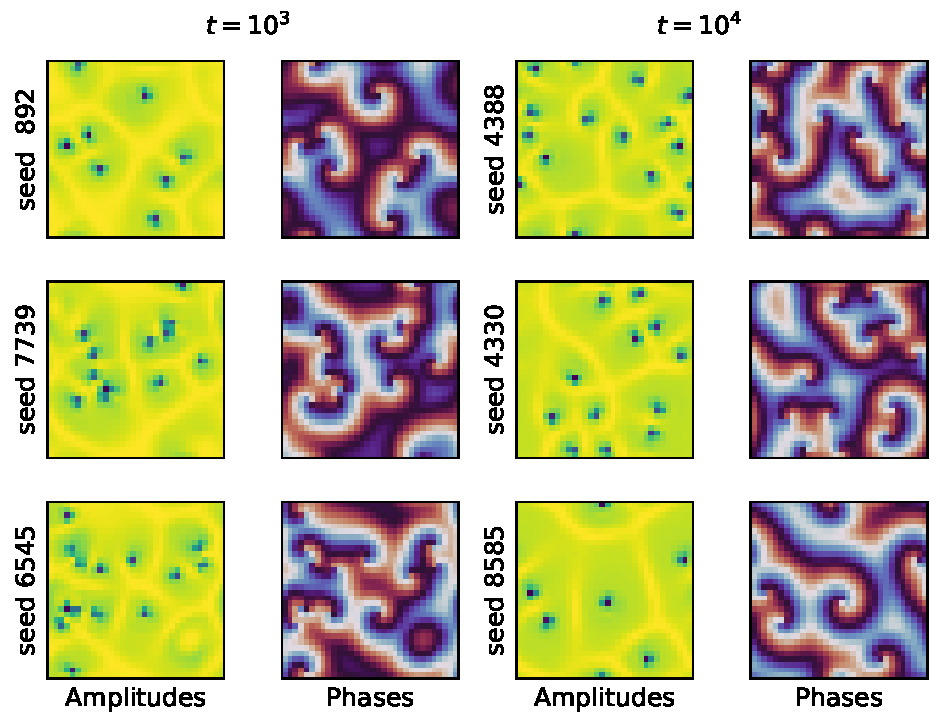
\includegraphics[width=1.0\linewidth]{../figures/samples_indistinguishable.pdf}
    \caption{Snapshots of randomly sampled transient ($t=10^3$) and steady-state CGL wavefunctions.
    Neither amplitudes nor phases show obvious inter-class differences.
    Note that vortices in the phase field center on low-amplitude defects (blue).}
    \label{fig:samples_indistinguishable}
\end{figure}

\section{Related work}
Accurately reconstructing transients remains challenging for machine-learning methods that build low-dimensional representations of complex dynamical systems,
such as dynamical mode decomposition (DMD) \cite{brunton2020machine}.
This is likely because transients are defined by non-stationarity,
that is, statistics that change over time \cite{said1984testing}.
Previous machine-learning studies of the CGL equation have thus focused on steady states:
Li and Liu et al. \cite{li2024measuring} used variational autoencoders to represent both simulated and experimental wavefunctions of the CGL,
but used the final records of long simulations to assure stationarity.
Similarly, Nicolaou et al. \cite{nicolaou2023data} study steady-state CGL wavefunctions to identify control parameters using the autoencoder-like
Sparse Identification of Nonlinear Dynamics (SINDy) model \cite{brunton2016discovering}.
Some studies have focused specifically on the properties of CGL transients,
such as Hermann et al., who use a modified DMD method to identify modes of transient CGL flows \cite{herrmann2021data}.
However, to our knowledge, no studies have focused specifically on distinguishing CGL transients and steady states.

Several studies have examined methods for transient detection in other dynamical systems, especially fluids.
Zhou et al. \cite{zhou2023development} test several machine-learning algorithms for distinguishing transients from steady states in the liquid-fueled molten salt reactors of nuclear power plants,
including recurrent neural networks, support vector machines, a decision tree, and $k$-nearest neighbors ($k$NN).
The $k$NN model was found to have the strongest performance.
However, nuclear power plants have fewer possible nonpathological steady states than the CGL equation, which can display a potentially infinite number of steady-state defect configurations \cite{aranson2002world}.
Meanwhile, Halford et al. \cite{halford2013standardized} use a simple feedforward neural network and a Gaussian mixture model to identify transients in electroencephalograms, which correspond to epileptic seizures.
Seizures exhibit spiral waves more similar to those of the CGL than the transients in nuclear power plants.
Published in 2013, Halford et al. did not use more recent convolutional neural networks;
moreover, the neural-network structure of the brain may make EEG signals more amenable to neural-network modeling than the CGL.
We thus study a wide range of models, not only neural networks.

\section{Data and features}
For simplicity and representative dynamics, we simulated Eq.~\ref{eqn:cgl} with $b=0$ and $c=1$ using previously published code~\cite{winterbottom2005complex,li2024measuring}.
Initial conditions were Gaussians of mean zero and standard deviation $10^{-4}$ at each pixel of a $32\times 32$ grid with periodic boundary conditions.
Wavefunctions were evolved using ETD2 exponential differencing with timesteps of 0.1~\cite{cox2002exponential}.
Wavefunctions were saved at times $10^3$ and $10^4$ for transient and steady-state snapshots.
We simulated $10^4$ independent initial conditions.
Our data thus consist of $10^4$ matched pairs of transients and steady states,
with each transient snapshot evolved for $(10^4-10^3)/0.1$ additional timesteps to obtain a matching steady-state snapshot.
As CGL wavefunctions are complex-valued,
we preprocess all snapshots into arrays of amplitudes and phases over simulation domains.
Amplitudes are normalized to the range [0, 1);
phases are expressed in units of cycles and thus intrinsically fall in the range [0, 1).
Transients are labeled 0 and steady-states are labeled 1.

For all models we used a random 60:20:20 split of training, development, and test data.
Splits were performed by matched pair, such that no pairs were shared between datasets.
For example, if the transient initialized with seed 8634 was allocated to the development dataset,
then the steady-state initialized with seed 8634 was also allocated to the development dataset.
Full training datasets thus consist of 6000 matched pairs.
To examine effects of matched-pair training data on model performance,
models were first trained using random halves of each matched pair (3000 unmatched transients and 3000 unmatched steady states for 6000 total samples),
which we term `unmatched halves.'
Models were then trained on 3000 randomly sampled matched pairs (6000 total samples), which we term `half matches':
only 3000 of 6000 matched pairs were used so that the total number of samples, 6000, would equal that of an unmatched dataset and permit fair comparison.
To examine effects of dataset size on model performance,
models were additionally trained on all 6000 matched pairs (12000 total samples), which we term `all matches.'
We posited that matched-pair training data would improve model performance,
as transients and steady states are more readily distinguishable to the human eye when presented as matched pairs (Fig.~\ref{fig:matched_pairs}).
To avoid dependence between matched samples,
halves of each matched pair were randomly dropped in development and test sets.
Development and test sets thus each consist of 1000 unmatched transients and 1000 unmatched steady states.

\begin{figure}
    \centering
    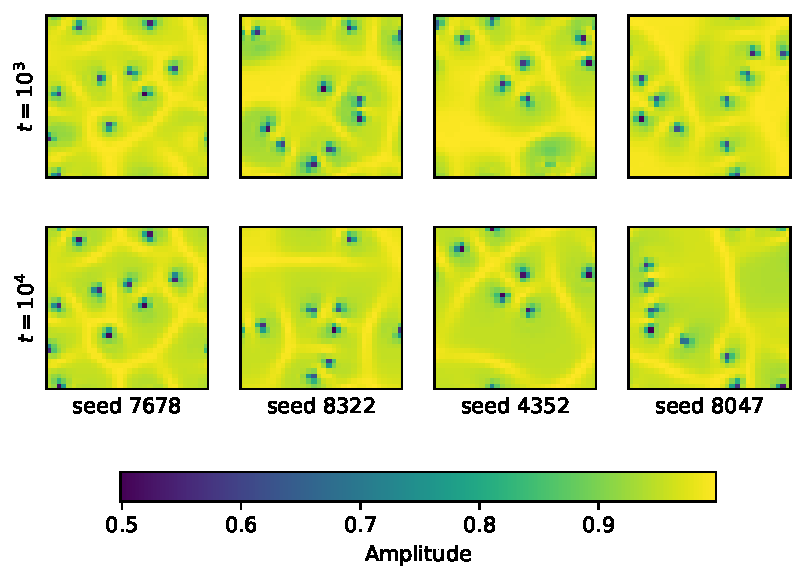
\includegraphics[width=0.9\linewidth]{../figures/matched_pairs.pdf}
    \caption{Transients and steady states are more readily distinguished in matched pairs.
    Transients exhibit slightly more low-amplitude defects (blue) and
    wider high-amplitude vortex-domain boundaries (yellow) than steady states.
    \label{fig:matched_pairs}
    }
\end{figure}

\section{Logistic regression}
\subsection{Method}
As a simple baseline, we classified our data using the \texttt{LogisticRegression}
class from the Python package \texttt{scikit-learn}~\cite{scikit-learn}.
In brief, this class implements the standard logistic regression hypothesis function
\begin{equation}
    h_\theta (x^{(i)}) = \frac{1}{1+\exp(-\theta^T x^{(i)})}
    \label{eqn:lr_hypothesis}
\end{equation}
with loss function
\begin{multline}
    J(\theta) = \frac{1}{C}\times\text{regularization}(\theta)-\\
    \frac{1}{N}\sum_{i=1}^N y^{(i)}\log h_\theta (x^{(i)})+(1-y^{(i)})\log [1-h_\theta (x^{(i)})]
    \label{eqn:lr_loss}
\end{multline}
where $\theta$ is a vector of learned hyperparameters,
$i$ indexes $N$ samples,
each $x$ is a vector of features (amplitudes and phases in our case) including a constant intercept,
each $y$ is the corresponding label,
and $C$ is a hyperparameter that controls the strength of the regularization.

\subsection{Experiments, results, and discussion}
We first tested the effects of dataset characteristics by training 
such models on each of our three training datasets
(unmatched halves, half matches, and all matches) using the default \texttt{lbfgs} solver (Limited-memory Broyden–Fletcher–Goldfarb–Shanno Algorithm)~\cite{lbfgs}.
Using approximations of the Hessian, \texttt{lbfgs} implements Newton's method to minimize
the loss function Eq.~\ref{eqn:lr_loss} for smooth regularizations.
We increased the maximum number of iterations from 100 to 3000 to assure convergence;
all other hyperparameters were set to defaults ($C=1$ with L2 regularization).
Evaluated on the development set, models trained on unmatched halves, half matches, and all matches
achieved accuracies of 0.67, 0.68, and 0.73, respectively.
Though dataset structure and size contribute only modest differences in accuracy,
we trained subsequent logistic-regression models on all matches to maximize performance.

To tune the bias-variance tradeoff, we trained further models using L1, L2, and no regularization.
Models with L1 regularization were trained using the \texttt{saga} solver~\cite{saga},
which implements stochastic gradient descent with a momentum term.
Models with L2 regularization were trained using \texttt{lbfgs} and models without regularization were trained using Newton's method.
We chose these solvers as the default \texttt{lbfgs} is suitable for L2 but unsuitable for L1;
\texttt{saga} is recommended by \texttt{scikit-learn} documentation for L1;
and, while neither \texttt{lbfgs} nor \texttt{saga} appears to converge without regularization,
Newton's method converges quickly and guarantees a globally optimal solution in that case.
Scanning through inverse regularization coefficients $C$
and evaluating trained models on the development set,
we found that the best-performing model achieved an accuracy of 0.761 using L2 regularization with $C=0.02$.

% \begin{figure}[h]
%     \centering
%     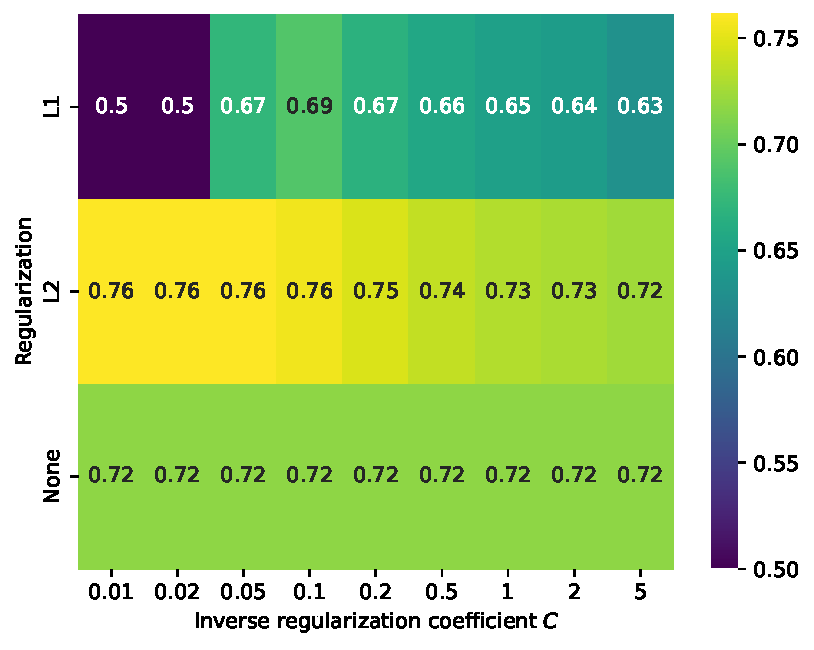
\includegraphics[width=1.0\linewidth]{../figures/lr_phase_diagram.pdf}
%     \caption{Logistic-regression accuracy varies with regularization form and strength.
%     The highest is obtained using L2 regularization with inverse coefficient 0.02.}
%     \label{fig:lr_phase_diagram}
% \end{figure}

Training ten such models and evaluating on the test set (which is balanced and does not contain matched pairs),
we observed that all models achieved the same accuracy, 0.7415.
While still unacceptably low, this accuracy is likely already greater than human accuracy on non-matched-pair data.
The $\texttt{lbfgs}$ solver appears to converge to the global optimum.
To interpret model decisions, we map parameters to the locations of their features on the $32 \times 32$ CGL simulation domain.
Parameters for amplitudes are uniformly negative, while parameters for phases are close to zero (Fig.~\ref{fig:lr_importances}).
This makes sense, as transients have more high-amplitude regions than their matched-pair steady states (Fig.~\ref{fig:matched_pairs}).
Negatively weighting high amplitudes decreases the hypothesis function Eq.~\ref{eqn:lr_hypothesis},
pushing the model toward class 0 (transient) predictions.
Phases seem to differ little between classes (Fig.~\ref{fig:samples_indistinguishable}).

\begin{figure}[h]
    \centering
    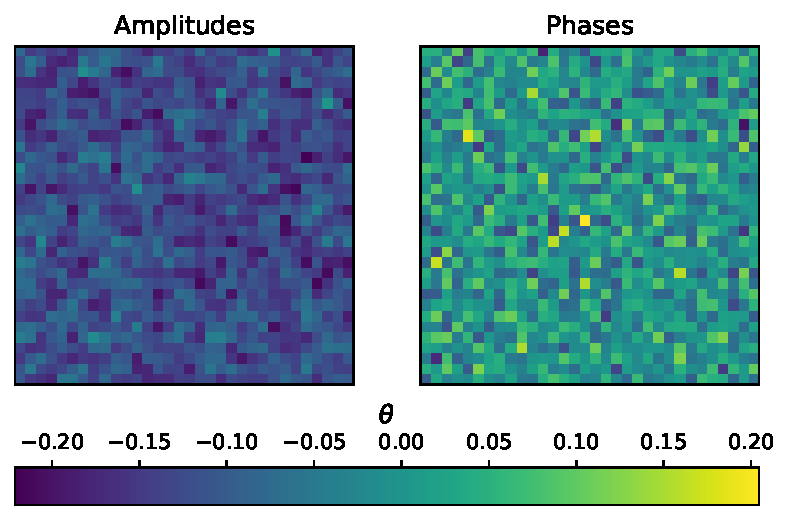
\includegraphics[width=1.0\linewidth]{../figures/lr_importances.pdf}
    \caption{Logistic regression learns negative weights for amplitudes and nearly zero weights for phases.}
    \label{fig:lr_importances}
\end{figure}

\section{Random forests}
\subsection{Method}
To assess whether ensembles of weak estimators might have better performance,
we then trained models to classify CGL wavefunctions using the \texttt{RandomForestClassifier}
class from the \texttt{scikit-learn} package~\cite{scikit-learn}.
This class implements a standard random forest using the CART (Classification and Regression Tree) algorithm~\cite{breiman1996bagging, breiman1984classification}.
Briefly, a hyperparameter number of decision trees are each trained using a bootstrap sample of the training data.
For a given tree at each step, a subset of the number of features (with cardinality equal to the square root of the total number of features)
is considered: the split that most decreases the Gini impurity is selected.
Trees are expanded up to a maximum depth that may be up to $\lceil\log_2 N\rceil$, where $N$ is the dataset size.
Predictions are assigned by a soft vote of trained trees.

\subsection{Experiments, results, and discussion}
As before, we first assessed effects of dataset characteristics by training models on each of our three training datasets.
All hyperparameters were set to defaults, with 100 trees per model each grown until all nodes reached zero impurity.
Evaluated on the development set, the models trained on unmatched halves, half matches,
and all matches achieve accuracies of 0.9525, 0.9485, and 0.9575, respectively.
As accuracies are similar across datasets, we train subsequent models on unmatched halves.
We note that these accuracies likely considerably exceed those of humans in distinguishing unmatched CGL transients from steady states.
Accuracies are already close to 1, suggesting that there is little overfitting.
We thus tune the number of trees without using pruning.
Scanning through forest sizes, we find that all evaluation metrics plateau around 128 trees (Fig.~\ref{fig:rf_metrics}).

\begin{figure}[h]
    \centering
    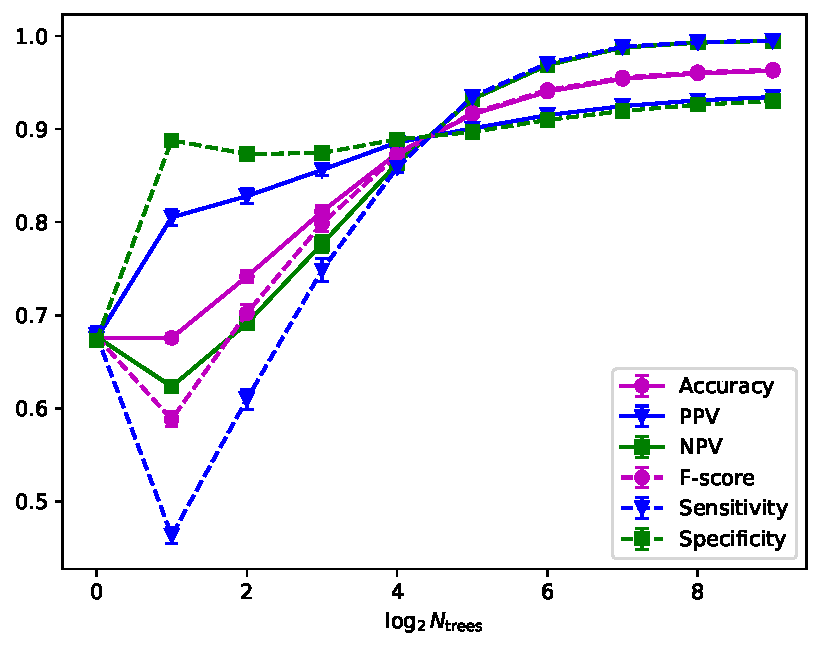
\includegraphics[width=1.0\linewidth]{../figures/random_forest_metrics.pdf}
    \caption{Random-forest metrics plateau at 128 trees.
    Error bars show 0.95 confidence intervals.}
    \label{fig:rf_metrics}
\end{figure}

We thus train and interpret a final model with 128 trees,
which achieves an accuracy of 0.9565 on the test set.
To interpret model decisions, we examine mean decreases in Gini impurity by feature.
Like logistic-regression models, random forests heavily weigh amplitudes but not phases.
This may be because transients show more extreme amplitudes (more defects and high-amplitude regions) than steady states.
We also perform error analyses by examining a random sample of misclassified wavefunctions.
Misclassified wavefunctions are visually similar to correctly classified wavefunctions (Fig.~\ref{fig:rf_misclassified}),
suggesting that different models may be required to achieve higher accuracies.

\begin{figure}[h]
    \centering
    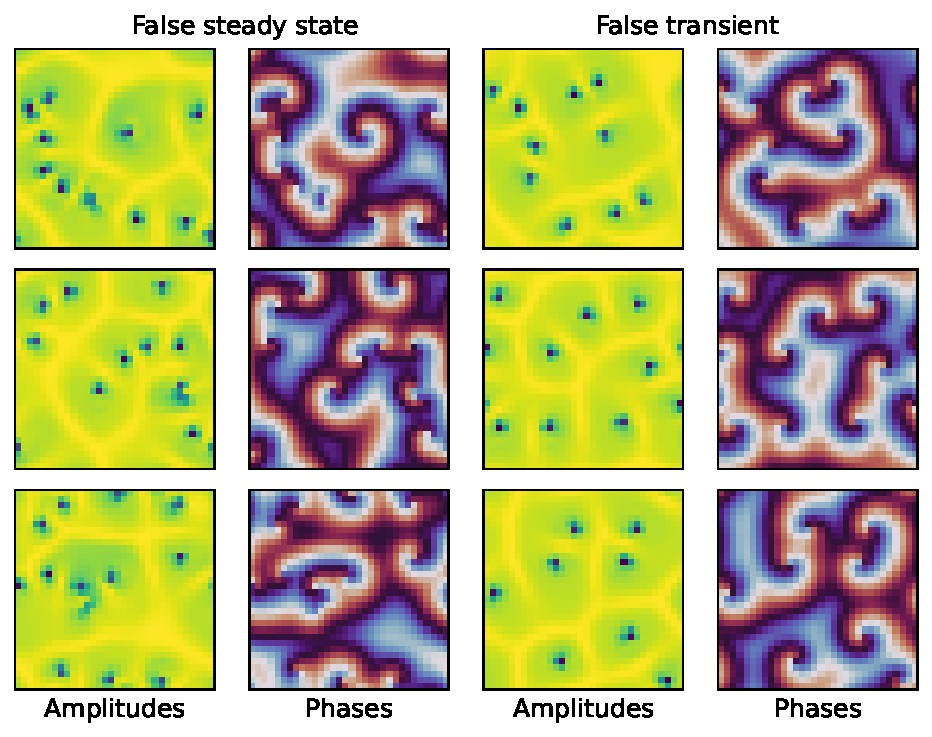
\includegraphics[width=1.0\linewidth]{../figures/rf_misclassified.pdf}
    \caption{Samples misclassified by random forests are not visually distinctive.}
    \label{fig:rf_misclassified}
\end{figure}

\section{Convolutional neural network}
\subsection{Method}
As data are images that may contain nonlocal data relevant to transient identification,
such as adjacent defects prone to anihilation, we next considered using convolutional neural network (CNN) models \cite{lecun2015deep}.
We built a feedforward CNN using the PyTorch package \cite{paszke2019pytorch}.
Convolutional layers were followed by ReLU activation layers, which were in turn followed by maximum pooling layers.
The output of the sequence of convolutional, ReLU, and maximum-pooling layers fed into a linear layer,
which was followed by another ReLU layer, a single-neuron linear layer, and a final sigmoid layer for outputting class probabilities.
All models were trained using the stochastic gradient-based Adam optimizer \cite{kingma2015adam} to minimize the binary cross entropy loss
\begin{equation}
    \ell = -\frac{1}{N}\sum_{i=1}^N y^{(i)}\log h_\theta (x^{(i)})+(1-y^{(i)})\log[1-h_\theta (x^{(i)})]
\end{equation}
where $h_\theta (x)$ denotes the probability of class 1 output by the CNN.
All models were trained for 50 epochs; the learning rate was decayed from 0.001 by a factor of 0.1 every ten epochs.

\subsection{Experiments, results, and discussion}
To check the overall suitability of CNNs for our task, we first trained a network with two two-channel convolutional layers with 3x3 kernels,
2x2 maximum-pooling layers, and a 16-neuron first linear layer.
Training was performed using 64-sample minibatches.
Evaluated on the development set, models trained on unmatched halves, half matches, and all matches achieved accuracies of 0.64, 0.66, and 0.70, respectively.
Ten such models were trained for each dataset: accuracy standard deviations were 0.05 for all datasets.
This performance is considerably poorer than that of logistic regression, necessitating hyperparameter tuning.

We tuned the number, number of channels, and kernel size of convolutional layers,
the use and non-use of batch normalization, and the number of neurons in the first linear layer.
For the channel numbers of the two or three convolutional layers, we used seven options ranging from $\{2, 2\}$ to $\{2, 8, 32\}$.
We used kernel sizes of 2x2, 4x4, and 8x8; as well as 2-, 8-, and 32-neuron first linear layers.
Four models were trained for each hyperparameter combination.
We found that the number of convolutional layers has little impact on performance.
In contrast, larger kernels, larger first linear layers, and batch normalization all improve performance.
However, the highest accuracy ($0.98\pm 0.01$) is achieved by models with $\{32, 8\}$-channel convolutional layers, batch normalization, and 2x2 kernels \ref{fig:cnn_accuracies}.

\onecolumngrid\
\begin{center}\
\begin{figure}[h!]\
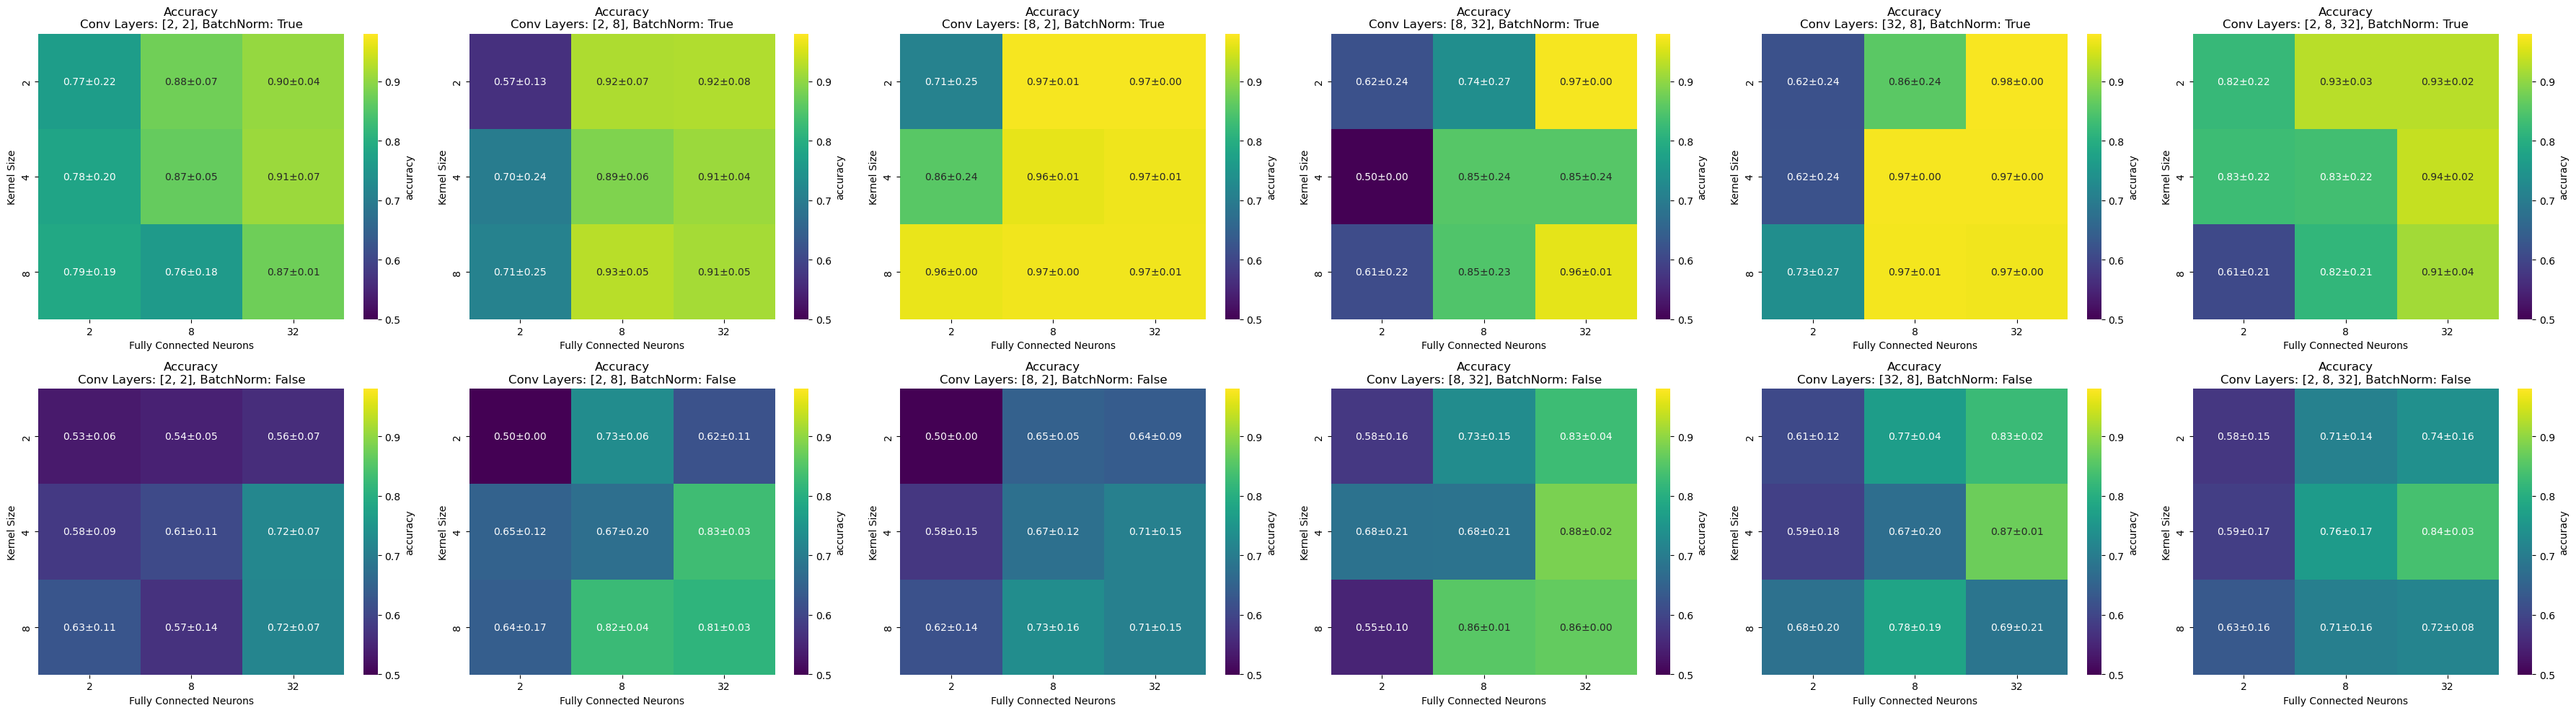
\includegraphics[scale=0.19]{../figures/B_new.png}\
\caption{CNN model accuracies vary with hyperparameter choice.}\
\label{fig:cnn_accuracies}
\end{figure}\
\end{center}\
\twocolumngrid\

Finally, we dissect the effects of convolutional-layer hyperparameters by visualizing the filters learned in the model with $\{8, 2\}$-channel convolutional layers,
batch normalization, a 32-neuron linear layer, and 4x4 kernels \ref{fig:kernels}.
Applied to sampled images, some filters pick out defects (filter 1) while others pick out vortex-domain boundaries (filters 2 and 7).
As defect density and domain size are respectively greater and lower in transient wavefunctions,
these features are likely important for classification.

\begin{figure}[h]
    \centering
    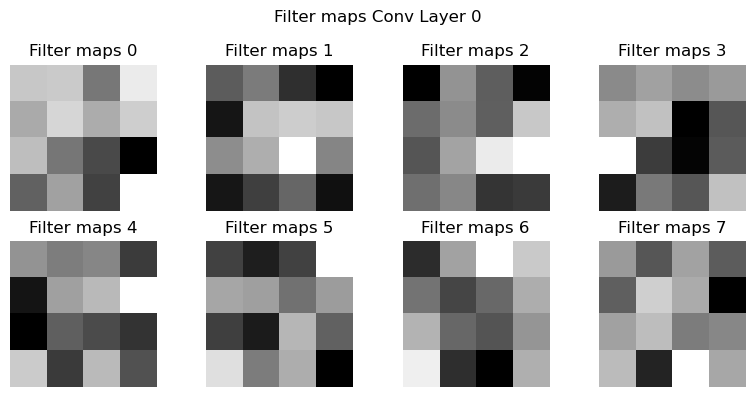
\includegraphics[width=1.0\linewidth]{../figures/D.png}
    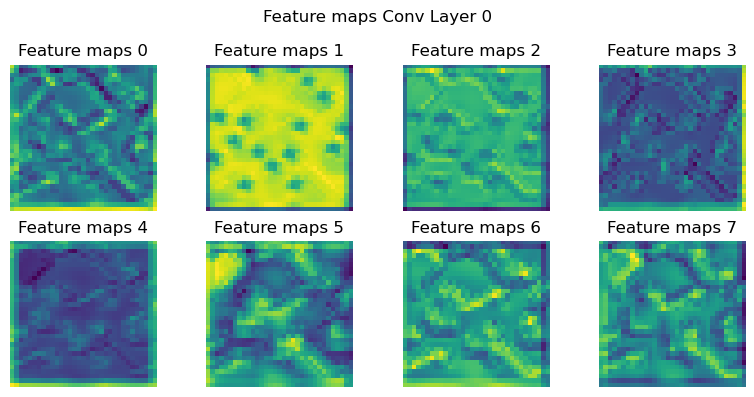
\includegraphics[width=1.0\linewidth]{../figures/C.png}
    \caption{Samples misclassified by random forests are not visually distinctive.}
    \label{fig:kernels}
\end{figure}

\section{Future work}
As the random forest forest classifier achieves high accuracy, it would be useful to examine whether other decision-tree ensembling methods might produce better performance.
In particular, AdaBoost~\cite{adaboost} could achieve superior performance with greater interpretability.
Similarly, the good performance of the CNN suggests that neural networks are suitable for this classification task.
We note that the number of convolutional layers seems to have little impact on performance.
Future research could examine whether convolutional layers are necessary at all;
non-convolutional neural networks may be equally capable of integrating nonlocal image features.

\section{Contributions}
C.W.J.L. and W.C.C. performed logistic regression analyses.
C.W.J.L. performed random forest analyses.
W.C.C. performed CNN analyses.
C.W.J.L. and W.C.C. wrote the paper.

\section{Acknowledgements}
C.W.J.L. was supported by was supported by the National Institute of General Medical Sciences of the National Institutes of Health through the Stanford Molecular Biophysics Training Program T32 grant 5T32GM136568-04.


\bibliography{main.bib}

\end{document}
